\documentclass[../monografia.tex]{subfiles}

\graphicspath{ {images/}{../images/} } % deixei aqui pra parar de aparecer erro, tava me irritando, só comentar de volta

\begin{document}



Para o desenvolvimento do projeto, dividimos as tarefas entre 3 áreas: Hardware, Firmware e Software. 

No \textbf{hardware} estará concentrado todo o desenvolvimento da eletrônica dos dispositivos que estarão nos nós da rede. 
O \textbf{firmware} será todo o software embarcado no dispositivo, desde a comunicação com o hardware até a comunicação sem fio, entre os dispositivos da rede e do dispositivo \textit{gateway} com a plataforma. 
O \textbf{software}, por fim, trata do desenvolvimento relacionado à plataforma onde os dados serão armazenados e apresentados. 

Por fim, foi desenvolvido um case mecânico simples, impresso em 3D, para proteger os componentes. 

\section{Hardware}

A partir das especificações técnicas, foi elaborado um novo diagrama de blocos. 

\begin{figure}[h]
    \centering
    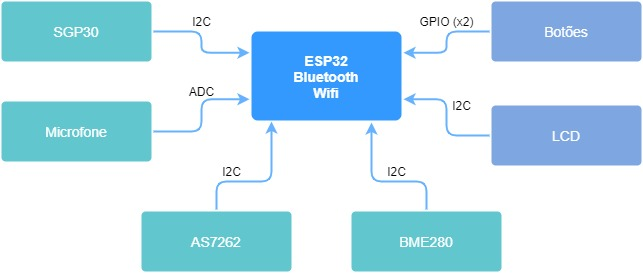
\includegraphics[width=12cm]{diagrama_hw_v1}
    \caption{Diagrama de Blocos de Hardware do Protótipo}
    \label{fig:img1}
\end{figure}

Quando possível, foram utilizados kits de desenvolvimento e módulos que nos permitisse uma validação mais rápida do hardware nessa fase inicial, permitindo avançar mais com o firmware e fazer testes em campo. 

O DevKitC do ESP32 possui integrado um USB, através do qual é possível alimentar os demais subcircuitos da placa, não existindo a necessidade de uso de bateria nessa etapa. 

\subsection{Esquemático}

Para o design do hardware, utilizamos o software de CAD de PCB \textit{Altium Designer 20} \cite{altium}. Foi utilizada a licença da empresa orientadora, sendo possível também conseguir uma licença gratuita para estudantes. Os arquivos estão disponíveis em \cite{git_hw}. 

A partir do diagrama de blocos, foi desenvolvido o esquema elétrico

\begin{figure}[h]
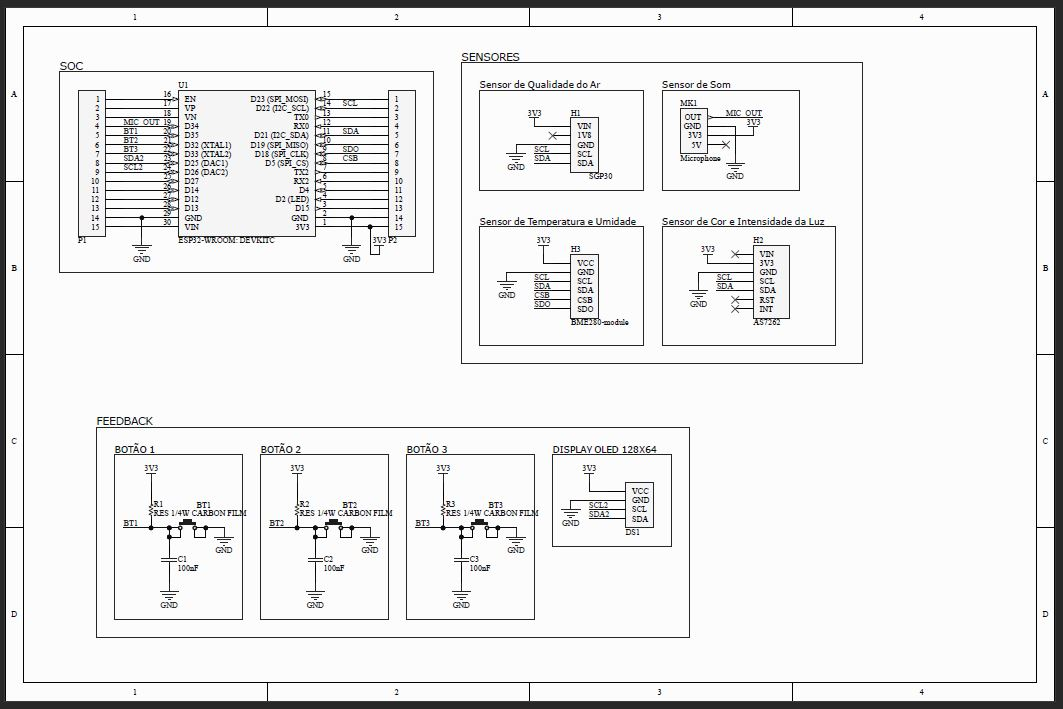
\includegraphics[width=\textwidth]{sch}
\caption{Esquemático do Protótipo}
\label{fig:img2}
\end{figure}

\subsection{PCB \textit{Printed Circuit Board}}

A partir do esquema elétrico foi feito um desenho de PCB (\textit{Printed Circuit Board}, ou Placa de Circuito Impresso), \textit{Single Layer}, e dimensões finais 60x70mm. 

\begin{figure}[h!]
\centering
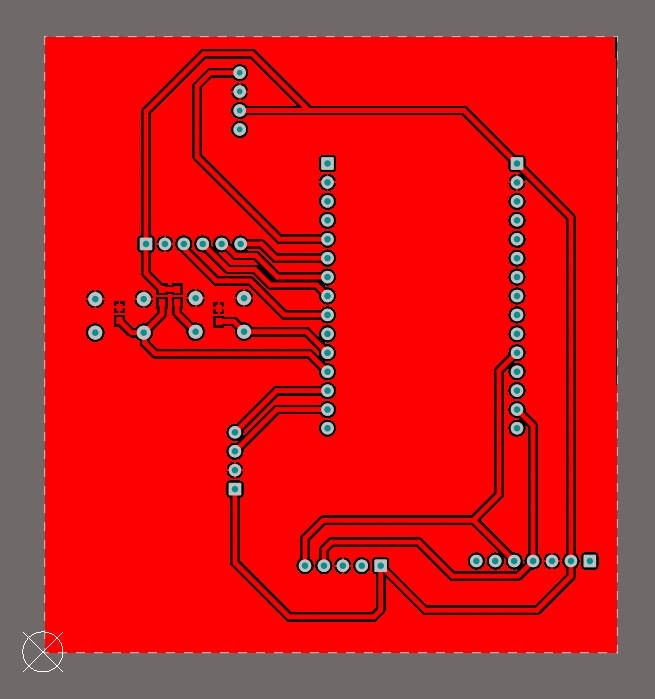
\includegraphics[width=8cm]{pcb_2}
\caption{Visão 2D da Camada Top Layer da PCB}
\label{fig:img3}
\end{figure}

%! atualizar o 3D que ta a versão 1
\begin{figure}[h!]
\centering
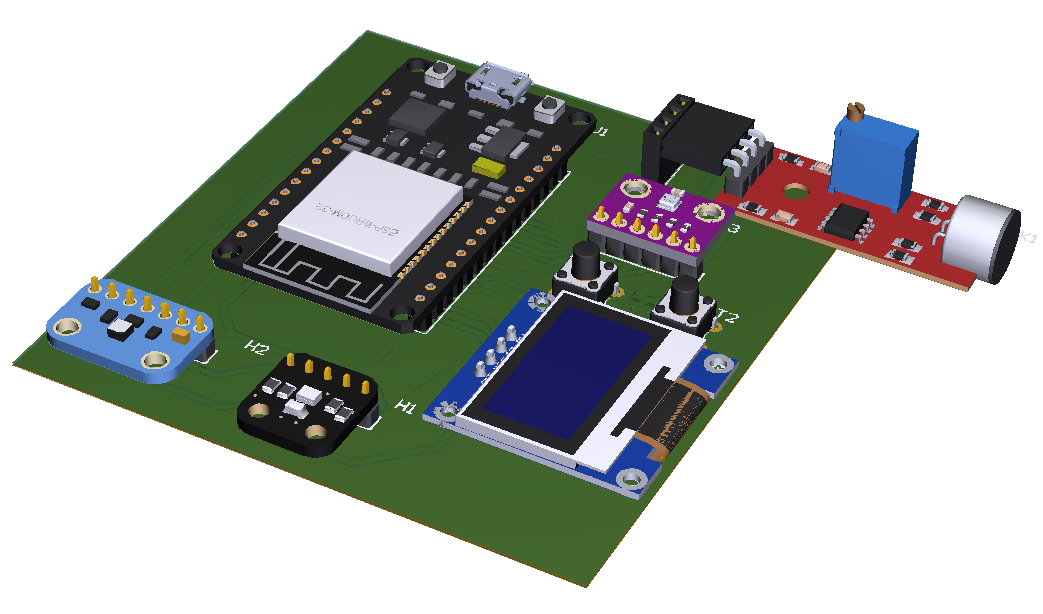
\includegraphics[width=10cm]{pcb}
\caption{Visão 3D da PCB}
\label{fig:img4}
\end{figure}

As placas foram fabricadas em fibra por uma fresadora CNC.

\begin{figure}[h!]
\centering
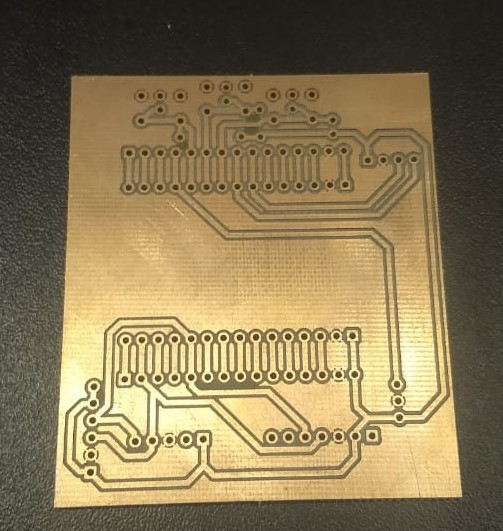
\includegraphics[width=10cm]{pcb-fresada}
\caption{PCB fresada}
\label{fig:img5}
\end{figure}

%? Montagem final da placa

\section{Firmware}

%! Pensar em como posicionar/quebrar arvore
\begin{figure}[h!]
	\centering
	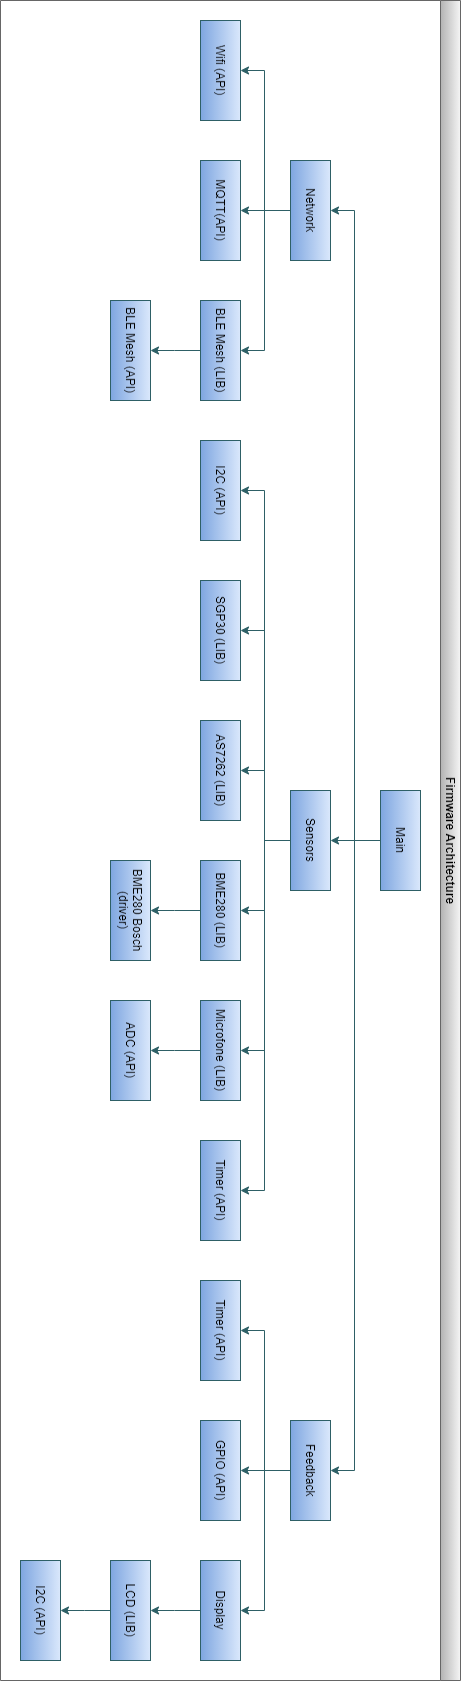
\includegraphics[height=0.9\textheight]{fw-arch}
	\caption{Arquitetura do Firmware dos dispositivos}
	\label{fig:fw-arch}
\end{figure}

\subsection{Sensores}

Para os sensores, desenvolvemos bibliotecas baseadas no ESP-IDF e validamos o funcionamento dos mesmos individualmente realizando algumas coletas de dados do ambiente. 

\subsubsection{BME280}

O BME280 é um sensor da Bosch que realiza medições de temperatura, umidade e pressão no ambiente. Possui 3 modos de operação: \cite{bme280}
\begin{itemize}
	\item \textit{sleep}: baixo consumo de energia, registradores podem ser lidos mas não realiza novas operações de medição.
	\item \textit{forced}: realiza uma medição, salva os resultados, e volta ao modo \textit{sleep}.
	
	\begin{figure}[h]
		\centering
		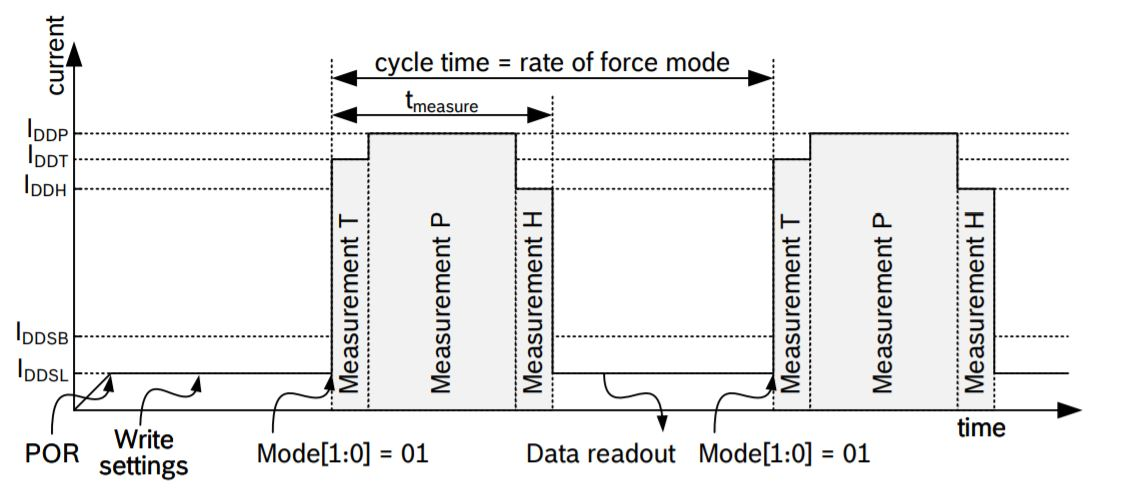
\includegraphics[width=12cm]{timing_bme280}
		\caption{Diagrama de tempos do modo \textit{forced}}
		\label{fig:time_bme280}
	\end{figure}

	\item normal: realiza medições periodicamente. O consumo durante o \textit{standby} entre medições é maior que o consumo no modo \textit{sleep}. 
\end{itemize}

O \textit{datasheet} recomenda que, para aplicações do tipo \textbf{monitoramento climático}, seja utilizado o modo \textit{forced}, com cerca de 1 medição por minuto. Assim, o sensor consumirá uma corrente de aproximadamente 0.16$\mu$A, sendo o modo de maior economia de energia. 

A Bosch Sensortech disponibiliza um driver para o BME280, com código fonte em C e disponibilizado abertamente\cite{bme280-driver}, que permite sua integração ao firmware em microcontroladores de qualquer fabricante. 
Utilizando o driver como base, desenvolvemos uma biblioteca para a utilização do BME280 no ambiente ESP-IDF, utilizando comunicação I2C, disponível

%todo: colocar estrutura da lib

%* Teste de validação 
%? manter?
% \begin{figure}[h]
% 	\centering
% 	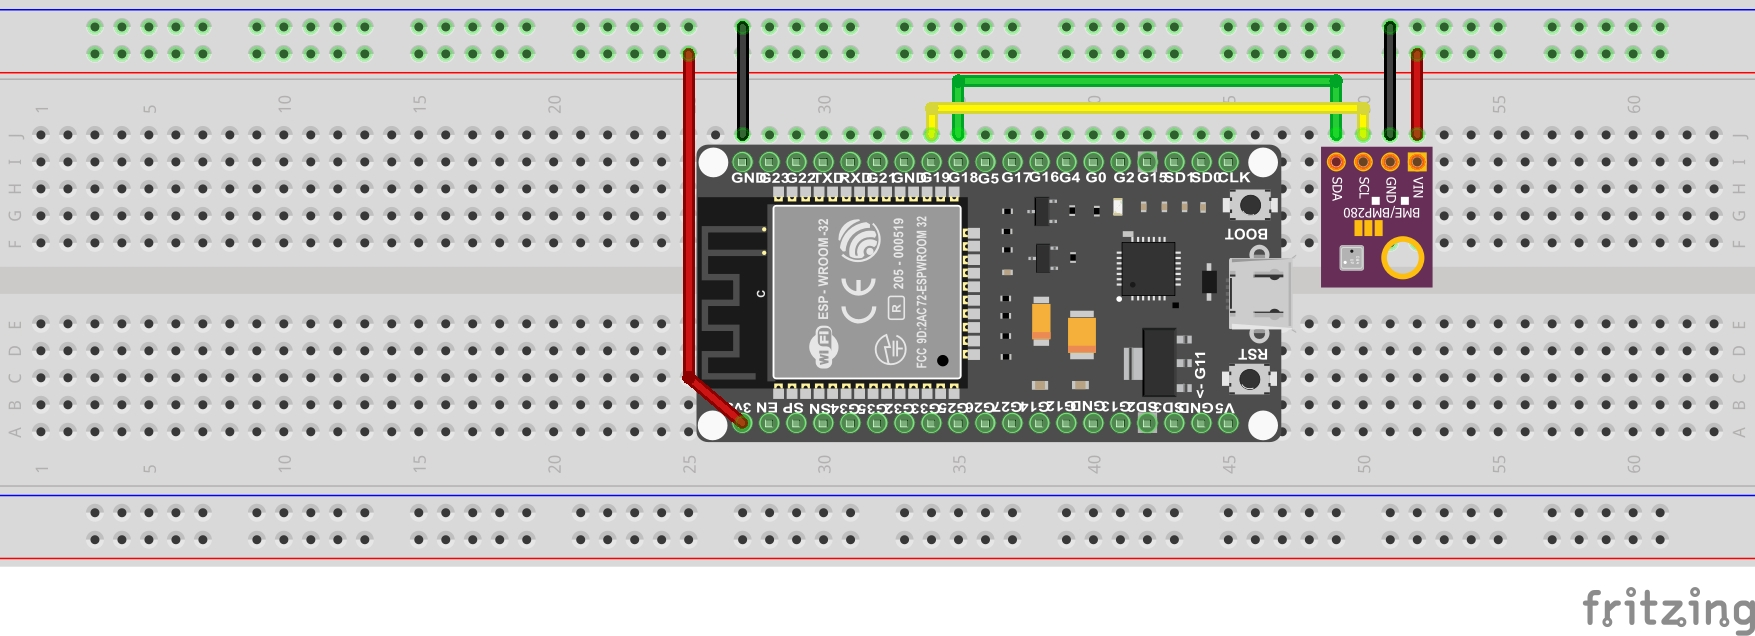
\includegraphics[width=12cm]{teste_bme280}
% 	\caption{Montagem na Protoboard do Teste com o sensor BME280}
% 	\label{fig:time_bme280}
% \end{figure}

\subsubsection{AS7262}
\subsubsection{SGP30}
\subsubsection{Microfone}
\subsection{Feedback}
\subsubsection{LCD OLED}
\subsubsection{Máquina de Estados}

Para a coleta do feedback, foi implementada a seguinte máquina de estados, seguindo um \textit{table-driven approach}.

%Máquina de Estados

%Estrutura do Código

\subsection{Bluetooth}
\subsubsection{Validação da Rede Mesh}

Visando validar a parte de comunicação sem fio utilizando BLE Mesh do ESP32 para o uso no projeto, uma rede simples com apenas 3 dispositivos foi desenvolvida. Dentre os dispositivos, 2 deles eram constituídos pelo microcontrolador escolhido conectados a de 3 LEDs cada um, e o terceiro um \textit{smartphone}. 

\begin{figure}[h]
	\centering
		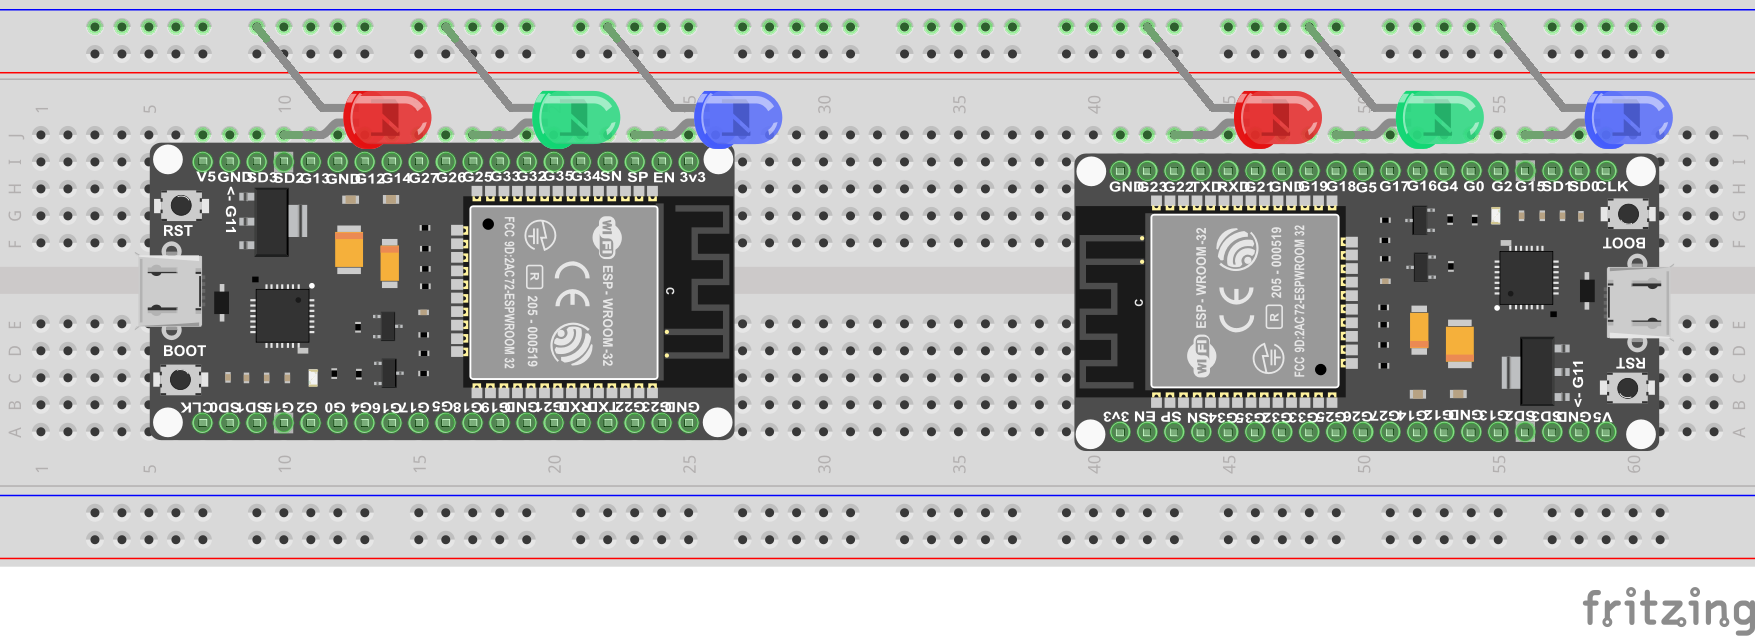
\includegraphics[width=.8\textwidth]{mesh_test}
		\label{fig:test}
		\caption{Montagem na Protoboard para o teste de Validação da Rede Mesh}
\end{figure}

Arquitetura da rede de testes criada:

\begin{itemize}
	\item Nó com microcontrolador ESP32: 3 elementos, cada um com o \textit{OnOff Server Model} \cite{ble-mesh-models} implementado, visando controlar o ligamento e desligamento de um LED.
	\item \textit{Smartphone}: utilizando o aplicativo nRF Mesh \cite{nrf-app}, usado para provisionar os outros nós e controlar a rede \textit{mesh}.
\end{itemize}

O teste completo aqui descrito pode ser visto em \cite{teste-ble-mesh}.

A partir do aplicativo citado, os outros dois dispositivos foram provisionados, criando a rede \textit{mesh}. Depois, foram criados 3 grupos diferentes:

\begin{itemize}
	\item \textit{Red Lights}: grupo em que os \textit{models} que controlam os LEDs vermelhos nos nós foram inscritos;
	\item \textit{Green Lights}: grupo em que apenas um dos \textit{models} que controlam LEDs verdes foi incrito;
	\item \textit{Red and Blue}: grupo em que tanto os \textit{models} de LEDs vermelhas quanto os de LEDs azuis foram inscritos.
\end{itemize}

O funcionamento da rede pode ser validado quando mensagens de \textit{On} e \textit{Off} eram enviadas em cada grupo e apenas os LEDs que deveriam receber a mensagem do respectivo grupo era acionado ou desligado.

Foi possível visualizar o a criação e o funcionamento de uma rede BLE Mesh na plataforma escolhida, bastando apenas modificar a lógica e parâmetros necessários para que as mensagens contenham os dados coletados pelos sensores do projeto e sejam enviadas para os dispositivos desejados.

\subsection{Wifi}
\subsubsection{MQTT}
\section{Software}
\section{Mecânica}

Foi projetado um case mecânico para proteger a eletrônica dos dispositivos, a ser impresso em 3D. 

O case é composto por duas peças, uma base, onde fica fixada a placa, e uma tampa onde ficam fixados o display OLED e os botões. As laterais abertas permitem que sejam feitos ajustes dos módulos com sensores sem afetar o funcionamento destes. 

\begin{figure}[h]
	\centering
	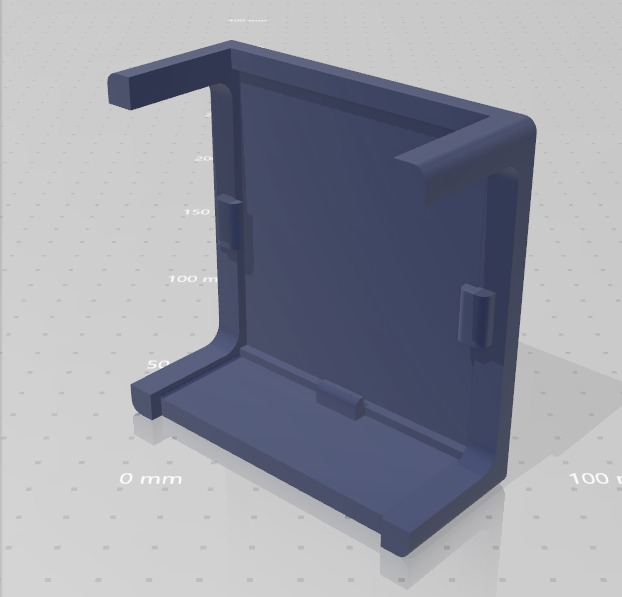
\includegraphics[width=0.6\textwidth]{mec-base.jpeg}
	\caption{Base do Case Mecânico}
	\label{fig:mec1}
\end{figure}

\begin{figure}[h]
	\centering
	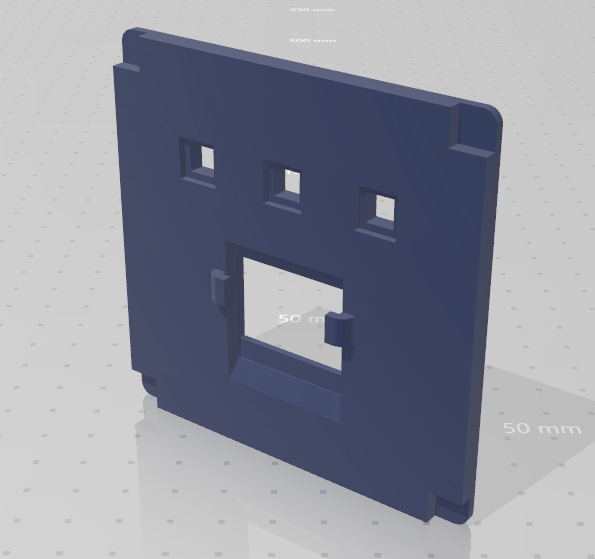
\includegraphics[width=0.6\textwidth]{mec-tampa.jpeg}
	\caption{Tampa do Case Mecânico}
	\label{fig:mec2}
\end{figure}

%* Montagem Final com Case

\end{document}